\documentclass[oneside,final,14pt,a4paper]{extreport}


%=====================================================================
%  BACHELOR THESIS PROPOSAL (REVISED after supervisor feedback)
%=====================================================================


\usepackage[T1]{fontenc}
\usepackage[utf8]{inputenc}
\usepackage[english]{babel}
\usepackage{tempora}

% Monospaced font: Courier (bold available via psnfss).
% The former manual \DeclareFontShape{OT1}{cmtt}{bx}{n}{...} was dead code:
% with \ttdefault=pcr it was never used, so it has been removed.
\renewcommand{\ttdefault}{pcr}

% Micro-typographic adjustments: reduce overfull lines caused by long
% identifiers and 14 pt setting, without changing the font size.
\usepackage{microtype}
\setlength{\emergencystretch}{2em}


\usepackage{vmargin}
\setpapersize{A4}
\setmarginsrb{2.5cm}{2.2cm}{2.2cm}{2.2cm}{0pt}{10mm}{0pt}{13mm}
\usepackage{setspace}
\setstretch{1.0}
\usepackage{indentfirst}
\parindent=1.25cm


\usepackage{amsmath,amsfonts}
\usepackage{amsthm}
\usepackage{upgreek}
\usepackage{bm}


\usepackage{xcolor}
\usepackage{graphicx}
\graphicspath{{figs/}}
\usepackage{float}
\usepackage{array}
\usepackage{multirow}
\usepackage{booktabs}
\usepackage{longtable}
\usepackage[font=singlespacing,labelfont=bf]{caption}
\usepackage{subcaption}
\usepackage{enumitem}


\usepackage{tikz}
\usetikzlibrary{positioning,arrows.meta}


\usepackage{csquotes}
\usepackage[backend=biber,style=ieee,autocite=inline]{biblatex}
\addbibresource{references.bib}
\DefineBibliographyStrings{english}{%
  bibliography = {References},}


\usepackage{chngcntr}
\usepackage{pdfpages}
\usepackage{placeins}
\usepackage{fancyhdr}


\captionsetup[table]{labelfont={normalfont}, name={TABLE}, labelsep={newline}}
\captionsetup[figure]{labelfont={normalfont}, name={Fig.}, labelsep=period}


\renewcommand{\thesection}{\arabic{section}}
\counterwithin{figure}{section}
\counterwithin{table}{section}
\counterwithin{equation}{section}
\setcounter{secnumdepth}{3}


\setlength{\headheight}{32.0976pt}

% Modern fancyhdr interface (replaces the deprecated fancyplain style,
% preserving the original header layout for this oneside document:
% left header = section mark, right header = page number, empty footer).
% \pagestyle{fancy}
% \fancyhf{}
% \renewcommand{\sectionmark}[1]{\markright{\thesection\ #1}}
% \fancyhead[L]{\bfseries\rightmark}
% \fancyhead[R]{\bfseries\thepage}
% \renewcommand{\headrulewidth}{0.4pt}


\usepackage{hyperref}
\hypersetup{colorlinks=true, linkcolor=black, citecolor=black, urlcolor=black}


\begin{document}

\begingroup
\setlength{\parindent}{0pt}
\setlength{\parskip}{0pt}

\begin{center}
    {\Large\bfseries
    Confidence-Aware Adaptive Verification of LLM Recommendations\\
    in Introductory Programming Tasks\par}
    \vspace{0.5em}
    {\normalsize Student: Lidia Davydova\par}
    \vspace{0.15em}
    {\normalsize Supervisor: Paolo Ciancarini\par}
\end{center}

\vspace{0.5em}

\begingroup
\small
\begin{minipage}{0.9\textwidth}
\noindent\textbf{Abstract.}
Large language models (LLMs) are increasingly used in programming
education, but their recommendations can be plausible yet incorrect,
so the quality of human--AI collaboration depends on
\emph{appropriate reliance}: accepting correct recommendations and
rejecting incorrect ones. Verification support can help users evaluate
recommendations, and introductory programming is well suited to it
because correctness can be checked through independent, execution-based
evidence such as tests, traces, and counterexamples. Providing such
evidence on every trial, however, introduces unnecessary interaction
cost. This thesis investigates whether a simple adaptive policy---gating
verification availability on the participant's \emph{prior-answer
confidence}---can reduce verification effort without degrading final-answer
accuracy relative to always-available verification. A within-subject
experiment ($N=60$) compares no-verification, static, and adaptive
conditions on a benchmark of 18 introductory Python tasks with frozen,
pre-validated Qwen3-8B recommendations balanced between correct and
incorrect. The two primary outcomes are final-answer accuracy (RQ1) and
total decision time as the primary measure of verification effort (RQ2).
Reliance measures, task type, and task difficulty are secondary or exploratory.
A pre-specified safety analysis examines the principal failure mode: confident
but mistaken participants for whom the gate withholds evidence, comparing their
outcomes with high-confidence static-verification trials. Expected contributions
are empirical evidence on the effort--quality trade-off of confidence-gated
verification, a reproducible benchmark and instrumented prototype, and an
analysis pipeline for the two primary outcomes.
\end{minipage}
\endgroup

\vspace{0.5em}
\endgroup

%=====================================================================
\section{Introduction and Research Problem}
%=====================================================================


Large language models (LLMs) are increasingly used in programming education
and software engineering to generate, explain, and debug code and to propose
answers to tasks \cite{Ma2024,Cambaz2024,Denny2024}. Because such systems can
produce plausible but incorrect outputs, the quality of the joint human--AI
outcome depends not only on model accuracy but on \emph{appropriate reliance}
\cite{LeeSee2004}: accepting correct recommendations and rejecting incorrect
ones. Over-reliance and under-reliance are the corresponding failures
\cite{PoursabziSangdeh2021,Vasconcelos2022}.


Verification support can help users evaluate recommendations, and programming
tasks suit it well: correctness can often be checked independently through
execution, tests, traces, or counterexamples---evidence grounded in the task
itself rather than in another LLM-generated justification. This matters
because explanations assist only when users can interpret them and connect
them to the recommendation, and simply providing more information does not
automatically reduce over-reliance
\cite{Bucinca2021,Vasconcelos2022,Bo2025,Schemmer2022}. Moreover, one can
only verify an answer one has the grounding to check \cite{Zhang2024Verify};
introductory programming provides exactly such grounding. However,
verification on every trial introduces unnecessary interaction cost, which
motivates providing verification evidence \emph{selectively}
\cite{CascadedLM2025}.


\subsection{Research Problem}

The research problem is how to provide verification support selectively, using
only information available before the correctness of the LLM recommendation is
known. The thesis investigates whether a simple adaptive policy, based
primarily on the user's \emph{prior-answer confidence}, can provide independent
verification support at lower effort than always-available verification, and
how verification effort trades off against decision quality. The focus is a
simple, interpretable policy---not a new LLM, a new verification algorithm, or
an optimisation method. The contribution is therefore not the threshold rule
itself; it is the controlled empirical evaluation of whether a simple
confidence gate can reduce verification exposure while preserving final-answer
accuracy and appropriate reliance compared with always-available and
no-verification baselines.

\subsection{Analytical Framing}
\label{subsec:framing}

The human--AI interaction is specified through an explicit \emph{escalation
rule} \cite{Ciancarini2027}: who recommends, who supplies independent
verification evidence, who decides, and what is recorded. The three
experimental conditions are three escalation policies within that single
specification, so the recommender, the evidence provider, the decider, and the
audit record are held fixed and only the routing of evidence changes.
Section~\ref{subsec:design} states the rule and its instantiation in the
study; Section~\ref{subsec:policy} states the confidence gate.

The rule is used as a specification device, not as a claim that the study
instantiates a full coordination model. There is a single decision-maker, a
frozen recommender that neither negotiates nor reallocates work, and no
multi-agent task allocation. The empirical question is when independently
produced evidence reaches the person who decides.


%=====================================================================
\section{Research Questions}
%=====================================================================


\textbf{RQ1 (accuracy, primary).} What is the effect of confidence-gated
adaptive verification on final-answer accuracy relative to (a)~always-available
static verification and (b)~no verification?

\textbf{RQ2 (effort, primary).} What is the effect of confidence-gated
adaptive verification on participant-level verification effort---primarily
total decision time, with evidence-examination rate and examination time as
secondary measures---relative to always-available static verification?

\textbf{RQ3 (exploratory).} How do the accuracy and effort effects of the
adaptive policy vary with prior-answer confidence, task type, and task
difficulty?

The thesis has two confirmatory tests. RQ1 is evaluated with a one-sided
non-inferiority test of adaptive versus static verification on final-answer
accuracy, against the pre-specified margin $\delta_Q$
(Section~\ref{subsec:quality}); the adaptive-versus-no-verification accuracy
contrast is reported as a supporting contrast with a 95\% confidence interval.
RQ2 is a one-sided superiority test of reduced total decision time for adaptive
versus static verification. Each primary test is conducted at one-sided
$\alpha=0.025$. The static-versus-no-verification contrast is reported
descriptively as a benchmark.

Reliance measures (Section~\ref{subsec:metrics}) are secondary and are used to
separate true reliance on the LLM from agreement with an answer the participant
already held. RQ3 is exploratory: task type, task difficulty, confidence
strata, and the premise check are reported with unadjusted estimates and
interpreted as hypothesis-generating rather than as confirmatory moderators.
Neither task type nor task difficulty is an input to the adaptive policy
(Section~\ref{subsec:policy}).

In addition, the \emph{confident-but-mistaken} case receives a dedicated
pre-specified secondary safety analysis (Section~\ref{subsec:blindspot}). It is
not an exploratory afterthought: because the gate withholds evidence exactly
when confidence is high, this is the boundary condition under which the policy
could cause harm, and it is examined with explicit estimands and a decision
rule for interpreting the result.


%=====================================================================
\section{Novelty and Contributions}
%=====================================================================


The novelty is \emph{not} the observation that confidence relates to reliance
on AI---miscalibration is well documented \cite{KrugerDunning1999,Bo2025} and
taken here as a premise---but the combination of elements usually studied in
isolation: (i)~confidence as a per-trial \emph{trigger} deciding \emph{when}
support is shown, rather than an outcome to be calibrated or an AI-side
uncertainty signal; (ii)~\emph{independent, execution-based} evidence (tests,
traces, counterexamples) rather than additional AI-generated explanations;
(iii)~a programming setting in which recommendations are pre-validated and
objective evidence exists; and (iv)~an explicit effort--quality trade-off
evaluation, treating verification effort as a first-class outcome
\cite{CascadedLM2025,Zhang2024Verify}.


The thesis is expected to contribute: (1)~trial-level empirical evidence,
analysed with mixed-effects models, on whether a simple confidence-based
policy reduces verification effort while preserving final-answer accuracy
(RQ1--RQ2); (2)~an explicit escalation rule that states who recommends, who
provides evidence, who decides, and what is recorded, and that treats the three
conditions as three escalation policies within one specification
\cite{Ciancarini2027}; (3)~a validated benchmark of 18 introductory Python
tasks with fixed, pre-validated LLM recommendations (balanced
correct/incorrect), task-type and difficulty labels, and verification data;
(4)~a reproducible prototype of the three conditions with complete logging,
including evidence examination; (5)~an analysis pipeline for the primary
outcome and effort measures.
The contribution is deliberately not a new LLM, a new algorithm, or a
tutoring system: the confidence gate is intentionally simple, and its value
lies in the controlled empirical comparison against always-available and
no-verification baselines in a reproducible human--AI interaction experiment.

%=====================================================================
\section{State-of-the-Art}
%=====================================================================

\paragraph{Trust and appropriate reliance.}
Trust in automation is classically defined as the attitude that an agent will
help an individual achieve a goal under uncertainty and in risky situations,
and the design goal is \emph{appropriate} reliance rather than maximal trust
\cite{LeeSee2004}. In AI-assisted decision-making, users frequently fail to
calibrate reliance to recommendation quality: over-reliance on incorrect
advice and under-reliance on correct advice persist even when additional
information about the model is available
\cite{PoursabziSangdeh2021,Chen2023}. Comparable miscalibration between
confidence and correctness is documented for human judgment itself
\cite{KrugerDunning1999}.

\paragraph{Explanations and cognitive forcing.}
Cognitive forcing functions, which compel deliberate engagement with AI
advice before it is accepted, can reduce over-reliance \cite{Bucinca2021}.
However, meta-analytic evidence finds no reliable benefit of explanations
over AI predictions alone \cite{Schemmer2022}, and experimental work shows
that explanations reduce over-reliance only when they are interpretable and
help users anticipate AI errors \cite{Vasconcelos2022}; interventions
evaluated with LLM advice similarly reduced over-reliance without improving
appropriate reliance overall \cite{Bo2025}. Because explanation-based
support may itself provide additional AI-generated information, this
motivates verification support grounded in independent, execution-based
evidence rather than additional AI text.

\paragraph{Verification and its cost.}
Correctness alone is an insufficient evaluation criterion: human scrutiny of
AI outputs is valuable but consumes time and effort, which motivates
frameworks that invoke human input selectively \cite{CascadedLM2025}.
Introductory programming supplies the grounding that verification requires:
executable reference answers, tests, and traces make objective evidence
available at decision time \cite{Zhang2024Verify}.

\paragraph{Confidence as a signal for adaptive support.}
Closest to this thesis, \cite{Bo2025} evaluate interventions for reliance on
LLM advice and find that interventions reduce over-reliance but generally
fail to improve appropriate reliance, while users' confidence is poorly
calibrated. The authors discuss confidence calibration as a design
implication. Related work adapts support to the user's trust state
\cite{SrinivasanAdjustForTrust}. Here, prior-answer confidence is instead an
\emph{input signal}: a lightweight trigger deciding \emph{when} independent
support is shown, leaving the user's internal state unchanged. The documented
relationship between confidence and correctness is taken as a premise: if
confidence carries information about correctness, it can also inform when
verification is worth its interaction cost---an effort dimension absent from
calibration-oriented work and a primary outcome here (RQ2).

\begin{table}[t]
\centering
\caption{Positioning relative to the closest lines of work.}
\label{tab:positioning}
\footnotesize
\begin{tabular}{@{}>{\raggedright\arraybackslash}p{2.7cm}>{\raggedright\arraybackslash}p{2.3cm}>{\raggedright\arraybackslash}p{2.9cm}>{\raggedright\arraybackslash}p{3.5cm}>{\raggedright\arraybackslash}p{2.7cm}@{}}
\toprule
Work & Signal & What is gated & Evidence & Primary outcome \\
\midrule
Bo2025 & None (intervention type) & Reliance intervention &
Accuracy or explanation & Appropriate reliance \\
Srinivasan et al. & User trust state & Explanation type; forced pause &
AI explanations & Inappropriate reliance \\
Zhang2024Verify & Decision difficulty & Feature explanation &
Feature attributions & Over-reliance \\
CascadedLM2025 & Model confidence and cost & Human review &
Model cascade & Cost and accuracy \\
This thesis & Prior-answer confidence & Independent execution evidence &
Tests, traces, counterexamples & Accuracy and effort \\
\bottomrule
\end{tabular}
\end{table}

Table~\ref{tab:positioning} makes the combination claimed as novel explicit:
each element exists separately, but no prior study gates \emph{independent,
execution-based} evidence on the decider's own prior confidence and treats
interaction effort as a primary outcome.

\paragraph{Coordination and governance of LLM-based systems.}
Because a language model can produce a fluent answer without guaranteeing that
it is correct, in scope, or compatible with other decisions, plausible but
unsupported output must be managed by the surrounding system rather than
trusted on fluency alone \cite{Ciancarini2027}. Recent work on agentic software
engineering argues that autonomy increases, rather than reduces, the need for
coordination: claims may need to be checked against artefacts, actions against
permissions, and decisions against explicitly assigned authority, and shared
artefacts, logs, tests, and approval points make decisions traceable
\cite{Ciancarini2027}. Coordination determines, among other things, the
escalation paths of a system: who supplies evidence, who decides, and under
whose authority. This motivates the explicit escalation rule adopted here
(Section~\ref{subsec:design}), in which independent execution-based evidence
replaces reliance on conversational
output alone.

\paragraph{LLM assistance in programming and research gap.}
LLMs are increasingly used for code generation, debugging, and explanation in
computing education \cite{Ma2024,Cambaz2024,Denny2024}, but can be plausible
yet incorrect, so users must evaluate recommendations critically. Prior work
establishes that intuition, explanation design, and decision difficulty shape
reliance \cite{Chen2023,Vasconcelos2022,Zhang2024Verify}; what remains
unknown is whether a participant's prior-answer confidence can serve as a
lightweight trigger for selectively displaying \emph{independent verification
evidence} after an LLM recommendation in introductory programming
tasks---the gap addressed here.


%=====================================================================
\section{Goal of the Thesis}
%=====================================================================

The goal of the thesis is to implement and empirically evaluate an
experimental system that provides selective verification support for LLM
recommendations in introductory programming tasks. The two primary outcomes are
final-answer accuracy and total decision time; the study tests whether a simple
confidence-based adaptive policy can reduce decision time while preserving
accuracy relative to an always-available (static) policy.

The project schedule is provided in Section~\ref{sec:workplan}.

\subsection{The Escalation Rule}
\label{subsec:design}

Coordination, in the account of Ciancarini \cite{Ciancarini2027}, determines
among other things the escalation paths of a system: who supplies evidence, who
decides, and under whose authority, so that correct and incorrect
recommendations are managed by the surrounding system rather than by
conversation alone. The study adopts that element as an explicit
\emph{escalation rule}. The rule does not add a new component; it makes
explicit the routing already implied by the design. Table~\ref{tab:escalation}
maps its parts onto the study.

The three experimental conditions are therefore \emph{three escalation policies
within the same specification}: only the escalation rule changes, while the
recommender, the evidence provider, the decider, and the audit record are held
fixed. Decision authority is never reassigned: the participant decides in every
condition, and only the flow of evidence is conditional. The rule is a
specification device rather than a claim that the study instantiates a full
coordination model: there is one decision-maker, a frozen recommender that
neither negotiates nor reallocates work, and no multi-agent task allocation.

\begin{table}[H]
\centering
\caption{The escalation rule and its instantiation in the study.}
\label{tab:escalation}
\small
\begin{tabular}{@{}>{\raggedright\arraybackslash}p{2.6cm}>{\raggedright\arraybackslash}p{7.4cm}>{\raggedright\arraybackslash}p{4.2cm}@{}}
\toprule
Role & Instantiation & Recorded artefact \\
\midrule
Recommender & Fixed, offline Qwen3-8B snapshot; no access to condition,
policy, or participant & Model hash, prompt, raw output \\
Evidence provider & Researchers; execution-based tests, traces, and
counterexamples derived from the task and reference answer, never from the
recommender & Verification artefacts and their expected outcomes \\
Decider & Participant records an initial answer, a prior-answer confidence
rating, and a final judgment & Responses, confidence, timestamps \\
Escalation rule & Static: evidence always; adaptive: evidence iff $c<\tau$;
no verification: never & Availability flag, policy decision, timestamp \\
Audit and record & Instrumented prototype logs the trial; the correctness
label is analysis-only and never shown & Trial-level log and analysis
dataset \\
\bottomrule
\end{tabular}
\end{table}


\subsection{Task Domain and Benchmark}
\label{subsec:answerspace}

The benchmark comprises 18 introductory Python programming tasks 
of three types: \emph{identify bug}, \emph{check against specification}, 
and \emph{select correct implementation}. ``Write or repair code'' 
tasks are excluded because they do not provide a sufficiently constrained 
response space for the primary reliance measures.

The benchmark metadata include task type, difficulty level, reference answer,
fixed LLM recommendation, recommendation correctness, and task-specific
verification data. The 18 LLM recommendations are balanced between nine
correct and nine incorrect recommendations. Correct and incorrect
recommendations are distributed across the three task types as evenly as the
benchmark construction permits.

\emph{Task difficulty.} Each task is assigned a difficulty level
(\emph{low}, \emph{medium}, or \emph{high}) before the main experiment
according to a predefined rubric based on code complexity, the number of
reasoning steps required, and the programming constructs involved. Difficulty
is descriptive metadata only: it is not an input to the adaptive policy and is
not used in the confirmatory analysis. Any use of difficulty in exploratory
reporting is labelled as such.

Each task has a closed-form response space that makes correctness 
and changes in the participant's answer well-defined. For \emph{identify bug}, 
the response consists of a binary bug-presence judgment and, when a bug 
is present, a line number identifying its location. Optional free-text 
explanations are recorded only for qualitative analysis. 
For \emph{check against specification}, the response is a binary 
\texttt{COMPLIANT}/\texttt{NOT\_COMPLIANT} judgment. 
For \emph{select correct implementation}, the response is an identifier 
corresponding to one of a fixed set of candidate implementations.

\emph{Canonical responses and equality.} Each task defines a canonical response
tuple and an accepted-equivalence set. For \emph{identify bug} the tuple is
(bug presence, line identifier), and a task may accept more than one line when
the bug spans a region; a judgment without a line is scored separately from a
judgment with a line. For \emph{check against specification} the tuple is the
binary judgment. For \emph{select correct implementation} the tuple is the
candidate identifier. Correctness and the equality relations used in
Section~\ref{subsec:metrics} are evaluated on the canonical tuple, never on
free text. The LLM recommendation is rendered through the same response widget
and with the same option labels as the participant's response, so that the
initial answer, the recommendation, and the final answer are directly
comparable and no letter remapping can occur.

\emph{Design and counterbalancing.} Each participant completes all 18 tasks,
with six trials assigned to each experimental condition. Each condition
contains two tasks of each of the three task types, and within each condition
three trials contain correct and three contain incorrect LLM recommendations,
with one of each per task type. Condition-to-task assignment uses a balanced
design with three rotation groups: across the three groups, each task appears
exactly once in each condition. Condition order is counterbalanced with six
sequences combining the three rotations and two orderings; task order within a
condition block is randomized per participant. Two practice trials precede the
experiment and are not analysed.

Because condition membership varies within task across participants and the
rotations are balanced, task-level heterogeneity is not systematically
confounded with the experimental condition, allowing task to be included as a
random effect in the analysis models.

\subsection{LLM Recommendation Specification}
\label{subsec:llm-spec}

All recommendations are generated offline before the experiment and frozen, so
every participant receives the same recommendation for a given task and
condition differences cannot be attributed to runtime sampling variance.

\emph{Model and configuration.} Recommendations come from a fixed local
snapshot of Qwen3-8B (8-bit GGUF, \texttt{Q8\_0}), run with thinking disabled
and a fixed decoding configuration. The model file, revision, quantization,
backend version, prompt template, and SHA-256 hash are archived with the
benchmark. Generation uses temperature 0.7, top-$p$ 0.8, top-$k$ 20, maximum
256 tokens, and zero frequency penalty, on a Tesla V100 (16~GB VRAM) with
128~GB RAM. Reproducibility is defined with respect to the archived model
artifact and outputs rather than bit-exact regeneration.

\emph{Prompt and output.} Each task prompt contains the task type, description,
code, a strict output schema, and an instruction to return only the answer. It
does not reveal the condition, policy, participant confidence, or intended
recommendation correctness. Outputs are parsed into the task's canonical
response space; unparsable outputs are regenerated.

\emph{Candidate selection.} Several candidates are generated per task and
scored against the reference answer. One recommendation is selected per task
before the study: nine correct and nine incorrect. Incorrect recommendations
must be objectively wrong but plausible to a novice; if the model produces no
suitable incorrect candidate, a documented minimal perturbation of a correct
answer may be used. Model-seeded items are flagged and excluded in a
sensitivity analysis, and the benchmark reports how many occur.

\emph{Validation and freezing.} Correctness is established automatically where
an objective procedure exists (execution, reference output, or predefined
tests) and otherwise by comparison with the reference answer. Two annotators
independently check correctness labels and rate the plausibility of incorrect
recommendations on a five-point scale; an incorrect item is retained only if
its mean plausibility is at least 3 and neither rating is below 2. Agreement is
reported with Cohen's $\kappa$, and disagreements are resolved by a third
annotator. The benchmark, prompts, labels, and selection decisions are then
frozen. Correctness labels are hidden from participants, the application, and
the policy module, and are used only in the analysis dataset.


\subsection{Verification Support and Effort Instrumentation}
\label{subsec:burden}

For each task, the verification mechanism is fixed before the experiment and is
identical across experimental conditions. The only manipulated factor is
whether the evidence is made available to the participant.

Verification is task-specific and independent of the LLM. For \emph{identify
bug} tasks, the system provides targeted tests or concrete counterexamples that
expose the bug and localise its effect. For \emph{check against specification}
tasks, it provides specification-based test cases with expected and actual
results. For \emph{select correct implementation} tasks, the candidates are
executed against a predefined test suite and the outcomes are displayed.
Artifacts are derived from the task specification and reference answer, not
from the recommender, and each has a predefined expected outcome. Two annotators
check that the evidence is correct, relevant, and sufficient; disagreements are
resolved by a third annotator, and the artifacts are frozen with the benchmark.

The evidence never states whether the LLM recommendation is correct and never
offers an alternative LLM judgment. It can nevertheless make the answer
derivable (for example, a test suite that only one candidate passes). Whether an
artifact is partial or decisive is recorded as benchmark metadata and used only
in exploratory interpretation, so that the study does not silently become a
test of compliance with decisive evidence.

Verification \emph{cost}---the intrinsic effort required to establish
correctness---is latent and is not claimed to be measured. The study measures
observable verification \emph{effort}, separated by level.
Table~\ref{tab:measures} defines the measures. \emph{Availability} refers to the
system, \emph{examination} to the participant, and the two time measures are
distinct. The measures are reported separately and are not combined into an
aggregate effort score.

\begin{table}[t]
\centering
\caption{Verification effort measures, their level, and their role.}
\label{tab:measures}
\small
\begin{tabular}{@{}>{\raggedright\arraybackslash}p{3.9cm}>{\raggedright\arraybackslash}p{1.9cm}>{\raggedright\arraybackslash}p{5.5cm}>{\raggedright\arraybackslash}p{2.7cm}@{}}
\toprule
Measure & Level & Definition & Role \\
\midrule
Verification availability (VAR) & System &
Share of trials on which evidence is offered & Manipulation check \\
Evidence-examination rate & Participant &
Share of available trials on which the panel is examined & Secondary effort \\
Evidence-examination time & Participant &
Seconds the evidence panel is active and focused & Secondary effort \\
Total decision time & Participant &
Seconds from recommendation to final judgment & Primary effort \\
Answer-change rate & Participant &
Final answer differs from initial answer & Descriptive \\
\bottomrule
\end{tabular}
\end{table}

The application records evidence-panel visibility, activation, dismissal,
scrolling, and final-judgment timestamps. A trial is classified as
\emph{evidence-examined} if the panel remains active for at least a fixed number
of seconds or the participant performs a predefined interaction with it; the
cut-off is fixed during the pilot. Evidence that is offered but not examined
still counts as available, so the adaptive condition is assessed both by how
often evidence was offered and by whether it was used when offered.


\subsection{Adaptive Verification Policy}
\label{subsec:policy}

The adaptive policy receives only one input: the participant's
\emph{prior-answer confidence} $c\in[0,100]$, defined as the confidence,
elicited before the recommendation is shown, that the participant's own
initial answer is correct. Verification is made available when

\[
c < \tau,
\]

where $\tau$ is fixed before the main experiment.

\emph{Why this signal.} Prior-answer confidence is chosen for three reasons.
First, it is available before the recommendation and therefore cannot be
contaminated by the advice. Second, it requires no model introspection or
additional AI-generated text, so the trigger remains independent of the
recommender. Third, low prior-answer confidence plausibly increases
susceptibility to advice \cite{YanivKleinberger2000}: participants who are unsure of their
own answer are more likely to defer to the recommendation, so the expected
value of independent evidence is highest exactly where the policy escalates
it. The relationship between confidence and correctness is treated as a
premise and tested separately (Section~\ref{subsec:premise}).

The policy does not receive the correctness of the LLM recommendation. Task
type and task difficulty are not policy inputs; they are retained as
experimental metadata and analysed only as exploratory factors (RQ3). The
policy therefore uses a single input---prior-answer confidence---and nothing
else.

\emph{Threshold.} The threshold is fixed during the pilot and before the main
experiment so that both the escalation and non-escalation branches are
exercised often enough to be analysed. The value is recorded in the
preregistration and is never estimated, optimised, or modified using
main-experiment data. Pilot participants are disjoint from main-experiment
participants, and pilot data are excluded from all main-experiment analyses.

The policy is deliberately minimal: its value lies in the controlled comparison
against the always-available and no-verification baselines (RQ1--RQ2), not in
the rule itself.

\subsection{Policy Premise Check}
\label{subsec:premise}

The policy assumes that prior-answer confidence carries information about the
probability that the participant's initial answer is correct. This assumption
is checked descriptively: a mixed-effects logistic model of initial-answer
correctness on confidence (scaled to $[0,1]$), with participant and task random
intercepts, is reported together with a calibration curve and the area under
the ROC curve. A positive association supports the premise; a weak association
is reported as a boundary condition on confidence gating. The check does not
determine or modify $\tau$, and the joint distribution of initial-answer
correctness and recommendation correctness is reported alongside it.

\subsection{Preserving Decision Quality}
\label{subsec:quality}

The adaptive policy is worthwhile only if it does not degrade decisions, so
decision quality is assessed explicitly rather than inferred from a
non-significant difference. The primary quality outcome is final-answer
accuracy; appropriate reliance is a secondary quality outcome
(Section~\ref{subsec:metrics}).

The central comparison is adaptive versus static verification, framed as a
\emph{non-inferiority} test on accuracy. The adaptive policy is not expected to
improve accuracy; it is expected to leave accuracy essentially unchanged while
verification is offered less often. Failing to detect a difference would not
establish that any difference is negligible.

Let $\Delta = \pi_{\mathrm{adaptive}} - \pi_{\mathrm{static}}$ be the difference
in the probability of a correct final answer, and let $\delta_Q>0$ be the
pre-specified non-inferiority margin, i.e.\ the largest acceptable loss in
exchange for reduced effort. The hypotheses are

$$
H_0:\ \Delta \le -\delta_Q
\qquad\text{versus}\qquad
H_1:\ \Delta > -\delta_Q .
$$

Rejecting $H_0$ establishes that adaptive verification is not worse than static
verification by more than $\delta_Q$. The margin is a substantive judgement
rather than an empirical estimate and is therefore fixed a priori in the
preregistration, together with its rationale, before any main data are seen. A
margin of ten percentage points is the working value; the final value is
confirmed in the preregistration and must be attainable at the target sample
size.

$\Delta$ is estimated as the marginal risk difference from the mixed-effects
accuracy model of Section~\ref{subsec:analysis}, with uncertainty obtained by a
parametric bootstrap over participants. Non-inferiority is declared when the
lower one-sided 95\% bound exceeds $-\delta_Q$. Raw proportions and their
confidence intervals are reported alongside the model-based estimate.

Adaptive verification is considered to preserve decision quality when it is
non-inferior to static verification on accuracy and reduces total decision time
(RQ2); the comparison with no verification provides a descriptive benchmark.

\subsection{Confident-but-Mistaken Participants (Policy Blind Spot)}
\label{subsec:blindspot}

The gate withholds evidence when $c\geq\tau$. Participants who are confident but
mistaken therefore receive no verification even when the recommendation is
incorrect. This is the principal failure mode of confidence gating, and the
thesis examines it directly rather than treating it as a descriptive footnote.

Two distinct harms are possible in the high-confidence stratum. First, a
\emph{missed correction}: the participant's initial answer is wrong and the
recommendation is correct, but no evidence is offered, so the error persists.
Second, a \emph{harmful adoption}: the initial answer is wrong and the
recommendation is also wrong, and the participant adopts it, producing a
confident error that the gate did not intercept. The second is the more serious
case, but both are reported, because high confidence can also make participants
less willing to defer and thus protect against the second harm while worsening
the first.

The pre-specified secondary safety analysis compares high-confidence trials in
the adaptive condition (evidence withheld) with high-confidence trials in the
static condition (evidence available) within the same participants and tasks.
The outcomes are (i)~final-answer accuracy and (ii)~the probability that the
final answer equals the LLM recommendation, reported separately for correct and
incorrect recommendations. Effects are reported descriptively as risk
differences with 95\% confidence intervals. The primary safety quantity is the adaptive-minus-static difference
in harmful adoption among high-confidence trials with an incorrect
recommendation and $A\neq L$; the corresponding accuracy difference is reported
alongside.

The interpretation rule is fixed before the main experiment. A safety margin of
ten percentage points is the working value: if the upper 95\% bound on the
increase in harmful adoption is below this margin and accuracy is not materially
lower, blind-spot harm is considered bounded; otherwise the gate is reported as
unsafe for this subgroup and the thesis conclusion is explicitly conditional on
that finding. This analysis is a safety check, not a third primary test, and it
does not use the primary alpha budget.

The design must contain enough high-confidence errors to support the analysis.
The pilot estimates the prevalence of high-confidence trials and of
high-confidence incorrect recommendations. The main study is required to yield
at least 40 high-confidence trials with an incorrect recommendation and
$A\neq L$ in each of the adaptive and static conditions; if the pilot predicts
fewer, $N$ is increased before preregistration. Exact counts, the realised confidence
distribution, and the number of high-confidence errors are reported, so a null
result cannot be mistaken for evidence of safety when the stratum is too sparse.
Second triggers or an audit fraction of high-confidence trials are discussed as
future work; the thesis evaluates the single-input policy and measures its
boundary behaviour.

\subsection{Participants, Recruitment, and Sample Size}
\label{subsec:participants}

The target population is Russian residents aged 18 or over who are enrolled in
or have completed at least one introductory programming course. Recruitment is
not restricted to the host university. Because the benchmark requires only basic
Python reading, control flow, and input/output knowledge, eligibility is
determined by the screening quiz rather than by institution, course grade, or
prior degree. Participants must be at least 18, report the required programming
background, and pass a short screening quiz of eight multiple-choice items on
Python reading, control flow, and basic input/output. The quiz is disjoint from
the benchmark, and the pass criterion (six or more correct) is fixed before
recruitment. Participants are excluded if they fail the screening, report prior
exposure to the exact benchmark tasks, or cannot complete the session for
technical reasons.

Recruitment is online and multi-channel: (i)~introductory programming courses
and mailing lists at the host university; (ii)~student communities and
course-alumni chats at other Russian universities, approached with permission;
(iii)~public programming-education communities on Telegram and VK; and
(iv)~snowball referral through participants. Advertisements state the
eligibility requirements, time commitment, compensation, and the fact that a
screening quiz must be passed. Course credit is offered where available;
otherwise participants receive a small fixed voucher. The target of $N=60$ is
planned across two academic terms, and participants are over-recruited by about
50\% to offset screening failures, no-shows, and withdrawals. Recruitment stops
when the preregistered target number of analysable participants has completed
the session or the recruitment window closes; excluded or withdrawn participants
are replaced. There is no optional stopping or outcome-dependent extension.
Participation is voluntary and requires informed consent.

\emph{Sample size.} The target is $N=60$ analysable participants. Each
participant completes 18 trials, giving up to 1,080 trial-level records and
about 360 records per condition, with approximately half of the records in each
condition containing a correct recommendation and half an incorrect one. The
six trials per condition are not treated as independent participant-level
replications; the analysis uses mixed-effects models with participant and task
random intercepts. For a within-participant accuracy contrast, 60 participants
give an expected 95\% confidence-interval half-width of roughly five percentage
points under plausible correlations, which is sufficient to assess a ten-point
non-inferiority margin. The pilot supplies variance components and the
confidence distribution; the final $N$ and the margin are fixed in the
preregistration before main data collection. Pilot participants are disjoint
from main-experiment participants and are excluded from all main analyses.

A complete session is expected to take 60--75 minutes, including instructions,
screening, practice, experimental trials, debriefing, and the demographic
questionnaire. All sessions are remote and self-administered in a web browser.

\emph{Recruitment and ethics feasibility gate.} Because recruitment and ethics
approval are the main schedule risks, the main experiment is not committed until
three checks are documented before preregistration.

\begin{enumerate}
\item \emph{Channel confirmation.} At least three active recruitment channels,
including at least one host-university course or mailing list, with documented
combined reach of at least 2,000 learners and permission to advertise in each
community. If this reach is not documented, additional channels or partner
universities are added before the target is fixed.
\item \emph{Expression of interest.} A short, non-binding sign-up survey (no
research data collected) is advertised through those channels before the main
study. At least 200 expressions of interest are required to reach 60 completions
under a conservative 30\% conversion rate after screening, scheduling, and
no-shows. If the response is lower, the channels are expanded and the target and
precision are re-planned before preregistration.
\item \emph{Ethics approval.} The protocol is submitted in early November, and
written approval from the institutional ethics body is required before any pilot
or main-experiment data are collected. The approval covers online recruitment
and remote data collection, including participants from outside the host
institution. A go/no-go review is held on 15 December. If approval is delayed,
the pilot and main experiment are shifted; no data are collected without
approval, and any reduction in sample size is reported with its precision
consequences.
\end{enumerate}

A recruitment log reports the numbers reached, screened, eligible, consented,
completed, and withdrawn at each stage, so that feasibility claims can be
checked against realised recruitment rather than assumed.

\subsection{Experimental Design and Procedure}
\label{subsec:procedure}
Three conditions are compared:

\begin{enumerate}
\item \emph{No verification}: the participant receives the LLM recommendation
but no verification evidence is provided.
\item \emph{Static verification (always available)}: verification evidence is
always made available after the LLM recommendation.
\item \emph{Adaptive verification}: verification evidence is made available
only when the participant's prior-answer confidence satisfies $c<\tau$.
\end{enumerate}

The verification mechanism is identical in all three conditions. Only the
display policy is manipulated. The benchmark composition and the
counterbalancing scheme are specified in Section~\ref{subsec:answerspace}: each
participant completes all 18 tasks, six per condition, with two tasks of each
type per condition and one correct and one incorrect recommendation per type
within each condition. Two practice trials precede the experiment.

All sessions use the same remote, self-administered procedure and the same
application. Participants may pause only between condition blocks. A researcher
is available for technical support but does not guide answers, so session mode
is constant and is not an experimental factor.

Each trial follows the sequence in Figure~\ref{fig:trial}.

\begin{figure}[t]
\centering
\begin{tikzpicture}[
  node distance=0.28cm,
  box/.style={draw, rounded corners=2pt, align=center, inner sep=3pt,
    minimum width=2.05cm, minimum height=0.95cm, font=\footnotesize},
  ar/.style={-{Latex[length=1.6mm]}}
]
\node[box] (task) {Task};
\node[box, right=of task] (ans) {Initial\\answer};
\node[box, right=of ans] (conf) {Prior-answer\\confidence};
\node[box, right=of conf] (llm) {LLM\\recommendation};
\node[box, right=of llm] (ev) {Verification\\evidence};
\node[box, right=of ev] (fin) {Final\\judgment};
\draw[ar] (task) -- (ans);
\draw[ar] (ans) -- (conf);
\draw[ar] (conf) -- (llm);
\draw[ar] (llm) -- (ev);
\draw[ar] (ev) -- (fin);
\node[below=0.4cm of ev, font=\scriptsize, align=center]
  {never $\mid$ always $\mid$ $c<\tau$};
\end{tikzpicture}
\caption{Trial sequence. The three conditions differ only at the evidence
step: never (no verification), always (static), or iff $c<\tau$ (adaptive).}
\label{fig:trial}
\end{figure}

The participant first provides an answer independently. The participant then
reports prior-answer confidence on a 0--100 scale. The fixed benchmark
recommendation is then displayed. Depending on the experimental condition,
verification evidence is either unavailable, always available, or made
available according to the confidence policy.

\emph{Interface and blinding.} In no-verification trials and in adaptive
trials with $c\geq\tau$, the verification affordance is displayed but
disabled, with the same wording in both cases (``No verification is available
for this trial''). The layout is therefore identical across conditions except
for whether the control is active, so participants cannot infer the condition
from the presence or absence of a panel. The exact threshold $\tau$ is not
disclosed. Instructions are scripted and delivered in the application. A
researcher is available via chat only for technical support, follows the
scripted protocol, and does not know the recommendation's correctness label;
participants are not told which recommendations are correct, and the application
never displays the label.

\emph{Confidence drift.} Because participants experience all three conditions,
they might learn that low confidence triggers evidence and adjust their reported
confidence accordingly. The analysis therefore compares the confidence
distribution across conditions and blocks, and the debrief asks whether
participants noticed a pattern or changed how they used the scale. Any evidence
of strategic reporting is reported as a limitation.

The participant subsequently records a final answer, which may confirm or change
the initial answer. The application never reveals the correctness label of the
recommendation; the label is stored only in the analysis dataset and is not
available to the participant-facing application or to the policy module.

For each trial, the system records the task identifier, task type, difficulty,
initial answer, prior-answer confidence, fixed recommendation, condition,
policy decision, recommendation correctness (analysis only), evidence
availability, panel events, examination status and duration, total decision
time, final answer, answer-change status, and timestamps. A trial is excluded
from timing analyses if the page loses focus for more than a pre-specified
duration; the rule is fixed before the main experiment.

\subsection{Evaluation Metrics}
\label{subsec:metrics}

The metrics are grouped into primary outcomes, secondary effort, reliance, and
safety measures, and descriptive transitions. The two primary outcomes are
final-answer accuracy (RQ1) and total decision time (RQ2). Reliance,
examination, and blind-spot safety measures are secondary. All reliance measures
use the initial answer recorded before the recommendation is shown, so reliance
on the LLM is separated from agreement with an answer the participant already
held.

Final-answer accuracy is the proportion of trials on which the participant's
final structured answer is correct according to the benchmark reference answer.

Let $A_i$ be the initial answer, $L_i$ the LLM recommendation, and $F_i$ the
final answer on trial $i$, all in the canonical structured response space
(Section~\ref{subsec:answerspace}). \emph{Agreement} is
$\text{Agree}_i=I(F_i=L_i)$, and \emph{LLM influence} (true reliance) is
$\text{Influence}_i=I(A_i\neq L_i \land F_i=L_i)$, which records a move toward
the recommendation from a different prior answer. Agreement in which the prior
answer already matched the recommendation is \emph{stable prior agreement} and
is not attributable to the LLM; the converse case is a \emph{switch away}.
Separating these cases prevents an already-held answer from being misread as
reliance. The change from $A_i$ to $F_i$ is a behavioural trace of reliance, not
by itself proof that the recommendation caused the change.

Reliance is reported as a secondary, descriptive outcome, broken down by
condition and recommendation correctness; no formal interaction model is part
of the bachelor scope. Over-reliance and under-reliance are reported
descriptively,
conditional on $A\neq L$: over-reliance is the share of incorrect
recommendations adopted when the prior answer differed, and under-reliance is
the share of correct recommendations not adopted when the prior answer differed.
Appropriate reliance---accepting a correct recommendation or rejecting an
incorrect one---is reported alongside, together with a stricter appropriate
updating rate restricted to $A\neq L$.

For the blind-spot analysis, two trial-level indicators are defined within the
high-confidence stratum $c\geq\tau$, both conditional on $A\neq L$:
\emph{harmful adoption} equals one when the recommendation is wrong and the
final answer equals it; \emph{missed correction} equals one when the
recommendation is correct and the final answer does not equal it. The
denominators are high-confidence trials with, respectively, an incorrect and a
correct recommendation and $A\neq L$. Both indicators are reported by condition
and used in the safety analysis of Section~\ref{subsec:blindspot}.

Total decision time is the number of seconds from the recommendation display to
the final judgment. Evidence-examination rate is the share of available trials
on which the evidence panel is examined, and evidence-examination time is the
seconds the panel is active and focused. The verification availability rate
(VAR) is the share of trials on which evidence is offered and is a manipulation
check rather than an effort outcome: it is zero in the no-verification
condition, one in the static condition, and the realised share of trials with
$c<\tau$ in the adaptive condition. The effort measures are reported separately
and are not combined into an aggregate score.

The smallest effect of interest for effort is fixed before the analysis: a 25\%
reduction in mean total decision time relative to static verification, or 60
seconds per trial, whichever is larger. A smaller difference is treated as
practically equivalent to static verification even if it is statistically
detectable.

Answer-change rate is the proportion of trials on which the final answer differs
from the initial answer. Changes are classified descriptively both by their
correctness transition relative to the reference answer and by whether they move
toward or away from the recommendation; the two classifications are distinct and
are not combined into a single outcome.

\subsection{Statistical Analysis}
\label{subsec:analysis}

The primary analyses are conducted at the trial level with mixed-effects
regression. Repeated observations from the same participant and the same task
are not treated as independent, so participant and task are included as random
intercepts. Because task--condition assignment is counterbalanced across
participants (Section~\ref{subsec:answerspace}), task characteristics are not
systematically associated with a condition. For binary outcomes the general
model is

$$
\operatorname{logit}\!\left(P(Y_{ij}=1)\right)
=
\beta_0
+
\boldsymbol{\beta}^{\mathsf{T}}\mathbf{X}_{ij}
+
u_i
+
v_j,
$$

where $Y_{ij}$ is the outcome for participant $i$ on task $j$, $\mathbf{X}_{ij}$
contains the fixed effects, and $u_i$ and $v_j$ are participant and task random
intercepts.

The primary predictor is condition, with no verification as the reference.
Planned contrasts compare adaptive with static verification and adaptive with
no verification; the static-versus-no-verification contrast is descriptive.

\emph{RQ1 (accuracy).} Final-answer correctness is modelled with the logistic
model above. The adaptive-versus-static contrast is evaluated as a
non-inferiority test against $\delta_Q$ (Section~\ref{subsec:quality}). The
marginal risk difference is obtained from the fitted model, with uncertainty
from a parametric bootstrap over participants; non-inferiority is declared when
the lower one-sided 95\% bound exceeds $-\delta_Q$. The adaptive-versus-no
contrast is reported as a supporting contrast with a 95\% confidence interval.
Raw condition proportions and confidence intervals are reported alongside.

\emph{RQ2 (effort).} Total decision time is right-skewed and non-negative, so it
is modelled with a generalized mixed-effects model with a Gamma family and log
link, with the same fixed effects and random intercepts. The adaptive-versus-
static contrast is a one-sided superiority test, reported as a ratio of expected
decision times with a 95\% confidence interval and compared with the smallest
effect of interest. Evidence-examination rate is analysed as a secondary
logistic outcome on available trials; examination time is analysed as a
secondary Gamma outcome on examined trials. These conditional measures are
interpreted descriptively rather than as causal effects of condition.

\emph{Secondary and safety analyses.} Reliance and blind-spot safety outcomes
are reported descriptively rather than with formal interaction models. LLM
influence, over-, under-, and appropriate reliance, harmful adoption, and
missed correction are summarised by condition and recommendation correctness,
with unadjusted 95\% confidence intervals. Within the high-confidence stratum
$c\geq\tau$, the adaptive-versus-static risk difference for harmful adoption
among trials with an incorrect recommendation is the primary safety quantity,
reported with a 95\% confidence interval and interpreted against the
pre-specified ten-point margin. These analyses are reported separately from the
confirmatory tests and are not used to adjust $\tau$.

\emph{Exploratory analyses.} Task type, task difficulty, prior-answer confidence,
the premise check, and confidence drift are reported with unadjusted estimates
and interpreted as hypothesis-generating. Task type and difficulty are not
policy inputs. These analyses are reported separately from the confirmatory
tests and are not used to modify $\tau$.

With 18 tasks, the task variance may be weakly identified. If the estimated
variance is effectively zero or the model fails to converge, the task random
intercept is dropped and the simpler model is reported. Missing final answers
are expected to be rare; the primary analysis uses available-case mixed models
under a missing-at-random assumption, and the amount of missing data is
reported. Timing exclusions follow the rule fixed before the experiment.

The two primary tests---adaptive-versus-static non-inferiority on accuracy and
adaptive-versus-static superiority on total decision time---are each conducted
at one-sided $\alpha=0.025$. Secondary, safety, and exploratory analyses are
reported with unadjusted confidence intervals; the blind-spot safety analysis
is interpreted against its pre-specified margin rather than as a confirmatory
test.
All primary hypotheses, contrasts, model specifications, exclusion rules, and
outcome codings are fixed in the preregistration before analysis of the main
data. Pilot data are excluded from all main analyses.

\subsection{Threats to Validity}
\label{subsec:threats}

\paragraph{Internal validity.}
The within-subject design exposes participants to all three conditions, so
order and learning effects are possible. Condition order is counterbalanced and
task order randomised, and condition-by-block interactions are checked. Demand
characteristics are reduced by scripted instructions, an identical disabled
control in all conditions, and a debrief about perceived patterns; confidence
drift is checked as described in Section~\ref{subsec:procedure}. Remote
self-administration introduces distractions; the application records focus loss
and excludes affected trials from timing analyses under a pre-specified rule.
Evidence can make the correct answer derivable, so whether an artifact is partial
or decisive is recorded and considered in exploratory interpretation
(Section~\ref{subsec:burden}).

\paragraph{External validity.}
Participants are Russian residents with introductory programming experience,
recruited online across universities and student communities, and the tasks are
short Python exercises with a closed response space. Online recruitment broadens
the institutional range but attracts self-selected, motivated learners, so the
sample is not representative of all novices. Conclusions may not transfer to
advanced programmers, open-ended code-writing tasks, or other languages. Only
one frozen model and one recommendation set are used, so the results describe
this model's recommendations rather than LLM advice in general.

\paragraph{Construct validity.}
Prior-answer confidence is a self-report and may be miscalibrated; the premise
check and calibration curve quantify how much information it carries. Total
decision time is a proxy for effort and includes reading and interface latency;
panel focus time is a proxy for attention. The study therefore reports several
effort measures rather than a single latent score, and does not claim to measure
intrinsic verification cost.

\paragraph{Statistical validity.}
Repeated trials are clustered within participants and tasks, so trial-level
independence is not assumed. Multiplicity is controlled for the two primary
tests, and the task sample is small enough that task-level effects are estimated
with uncertainty; the model simplification rule is pre-specified. The
non-inferiority conclusion is bounded by the a priori margin, and the sample is
justified by the precision of the primary contrasts rather than by a descriptive
floor. The blind-spot safety analysis is bounded by the number of
high-confidence errors; the design sets a minimum count and reports the realised
stratum size, so a sparse stratum is not interpreted as evidence of safety.

\subsection{Expected Software Artefacts}

The thesis will deliver:

\begin{itemize}

\item a documented escalation rule defining the recommender, the
evidence provider, the decider, the escalation condition, and the audit record
(Section~\ref{subsec:design});

\item a frozen benchmark containing 18 introductory Python tasks;

\item structured task metadata including type, difficulty, reference answer,
fixed LLM recommendation, and recommendation correctness;

\item the archived Qwen3-8B model specification, artifact hash, inference
configuration, prompts, candidate generations, and validation records;

\item the experimental web application;

\item the execution-based verification module;

\item a configurable confidence-based policy module;

\item structured experimental logging including evidence availability,
examination status and time, and total decision time;

\item the frozen benchmark-generation and validation scripts;

\item the statistical analysis scripts implementing the pre-registered
mixed-effects models;

\item recruitment and feasibility records, including channel confirmations and
reach, the expression-of-interest summary, and the recruitment log; and

\item documentation sufficient to reproduce benchmark generation,
experimental execution, and statistical analysis.

\end{itemize}


%=====================================================================
\section{Detailed Work Plan and Schedule}
\label{sec:workplan}
%=====================================================================


The work is planned from October 2026 to mid-May 2027. The required
deliverable is the bachelor's thesis. Publication of a research paper is an
optional aspiration that would build on the thesis if time permits, but it is
not a required outcome of the project.


\small
\begin{longtable}{>{\raggedright\arraybackslash}p{7.4cm}>{\raggedright\arraybackslash}p{2.0cm}>{\raggedright\arraybackslash}p{5.2cm}}
\caption{Work plan and schedule}
\label{tab:workplan} \\
\toprule
\textbf{Phase and activities} & \textbf{Period} &
\textbf{Deliverable / milestone} \\
\midrule
\endfirsthead


\toprule
\textbf{Phase and activities} & \textbf{Period} &
\textbf{Deliverable / milestone} \\
\midrule
\endhead


\bottomrule
\endfoot


1. Literature review and research design:
systematic study of appropriate reliance, verification cost, human--AI
interaction, confidence-aware support, and LLM assistance in programming;
completion of the bibliography &
October 2026 &
Annotated bibliography; refined research gap and research questions \\


2. Finalisation of the experimental design:
operational definitions, hypotheses, primary and secondary metrics,
confidence-based policy, and statistical analysis plan &
1--15 November 2026 &
Draft protocol and analysis plan \\


3. Benchmark construction and LLM recommendations:
selection of 18 introductory Python tasks, categorisation, difficulty
assessment, reference-answer validation, offline generation and validation of
recommendations (9 correct / 9 incorrect), and task-specific verification
evidence &
1--30 November 2026 &
Validated benchmark with frozen recommendations (M2) \\


4. Prototype implementation:
participant interface, task manager, fixed recommendation module, verification
module, adaptive policy, counterbalancing procedure, and experiment logger
including evidence-examination logging &
December 2026 &
Functional experimental prototype (M3) \\


5. Ethics approval, pilot, and protocol freeze:
ethics submission in early November and written approval before any pilot or
main data; confirmation of at least three recruitment channels with documented
combined reach of 2,000 learners and an expression-of-interest survey of 200;
15 December go/no-go review; pilot testing
of task clarity, interface usability, logging quality, confidence elicitation,
and calibration of the confidence threshold $\tau$ and the examination cut-off;
precision check for the primary contrasts and the high-confidence error count;
pre-registration &
November 2026--January 2027 &
Ethics approval; confirmed recruitment pool; frozen configuration
($\tau$, $\delta_Q$, $N$) and registered protocol (M4) \\


6. Main experiment:
online recruitment until the preregistered target sample is reached
(provisionally $N=60$ analysable), counterbalanced assignment, remote data
collection, recruitment log, monitoring of exclusions, quality control &
February 2027 &
Complete and anonymised trial dataset (M5) \\


7. Data analysis:
data cleaning, descriptive statistics, mixed-effects models for accuracy and
total decision time, descriptive secondary examination, reliance, and
blind-spot safety analyses, plus exploratory premise and confidence-drift
checks &
March 2027 &
Reproducible analysis scripts and preliminary results (M6) \\


8. Thesis writing:
writing the methods, results, discussion, limitations, and conclusion;
tables and figures; internal revision and proofreading &
March--April 2027 &
Complete thesis draft (M7) \\


9. Thesis finalisation:
final revision, formatting, reference checking, documentation of the software
artefacts, and supplementary materials &
By 15 May 2027 &
Submitted bachelor's thesis (M8) \\


10. Optional extension:
if time permits, preparation of a research paper from the thesis (an
aspiration, not a required outcome) &
After 15 May 2027 &
Optional paper draft \\


\end{longtable}
\normalsize

\paragraph{Principal risks.}
Recruitment is the largest risk. The design mitigates it with multi-channel
online recruitment across Russian universities and student communities,
documented combined reach of at least 2,000 learners, a pre-study
expression-of-interest survey of 200, rolling recruitment across two terms, and a
recruitment log; if the target is not met, the achieved precision is reported
rather than the intended precision. Ethics approval is the other schedule risk:
submission is in early November, approval is required before any pilot or main
data, and a go/no-go review on 15 December triggers a schedule shift rather than
data collection without approval. Benchmark construction and
annotation may take longer than planned; the four-week slot has no dependent
downstream task until the prototype is complete. Technical logging failures are
mitigated by a pilot and by server-side logging of every trial. If the pilot
indicates that the threshold is poorly placed, $\tau$ is recalibrated before
preregistration and the change is documented.

%=====================================================================
\section{References}
\printbibliography[heading=none]


\end{document}